\documentclass{article}
\usepackage{appendix}
\usepackage{graphicx}
\usepackage{pgfplotstable}
\usepackage{listings}

\title{HugeTLB Improvement to Reduce Post-Boot Allocation Failures}
\date{2016-02}
\author{Joshua Nicolas Verburg-Sachs}

\begin{document}
	\pagenumbering{gobble}
	\maketitle
	\newpage
	\pagenumbering{arabic}
	\tableofcontents
	\newpage

	\section{Preamble}
		This research was inspired by many frustrated attempts to utilize the excellent huge page facilities of the Linux kernel during runtime. Huge pages are a mechanism whereby the Linux kernel can allocate memory not in 4kb pages (or whatever your distribution uses) but page sizes ranging from many megabytes to a gigabyte or more (though we touch only on the megabyte sized pages in this paper). This gives a variety of advantages, one of the most important being a reduction in the number of page entries that the kernel must manage for your executable. This can, for example, significantly increase the speed of large mmaps and munmaps.

Most of the current use cases and documentation stipulate that you should only attempt to allocate huge pages immediately after boot, in order to avoid (very common) failures due to memory fragmentation and memory use by other executables. However this is not always a convenient option and in some situations (such as real time systems with uptime requirements) it is basically untenable.

Therefore, this paper will describe a method whereby the Linux kernel can be improved to more robustly allocate huge pages during runtime, even when other applications have consumed a significant amount of available memory.

\section{Amble}
	There are two primary causes to hugepage allocation failure. In order to illuminate them and discuss the solution we will describe the original algorithm here:
\begin{figure}
\lstinputlisting[language=C, firstline=967, lastline=987]{./hugetlb.c.orig}
\end{figure}
\ref{figure:Original Code Block}

\section{Mosey}
Below are two figures which describe 6 different scenarios for the default and new allocation method (hereafter called aggressive). The scenarios are simply a set of configuration options for the test run in question. These options are as follows: 
\begin{itemize}
	\item Aggressive: Whether to use aggressive alloc.
	\item Set: The number of pages to allocate.
	\item Grab: Whether to cause the test application to allocate memory (to disrupt hugepage allocation), and how much if so.
	\item  Iterations: How many times the test application should attempt to set the number of huge pages. In all test runs this was 10, as it proved sufficient for demonstrating performance.
	\item Reset: Whether to re-set the number of hugepages to 0 after each iteration.
\end{itemize}

\begin{figure}[h!]
	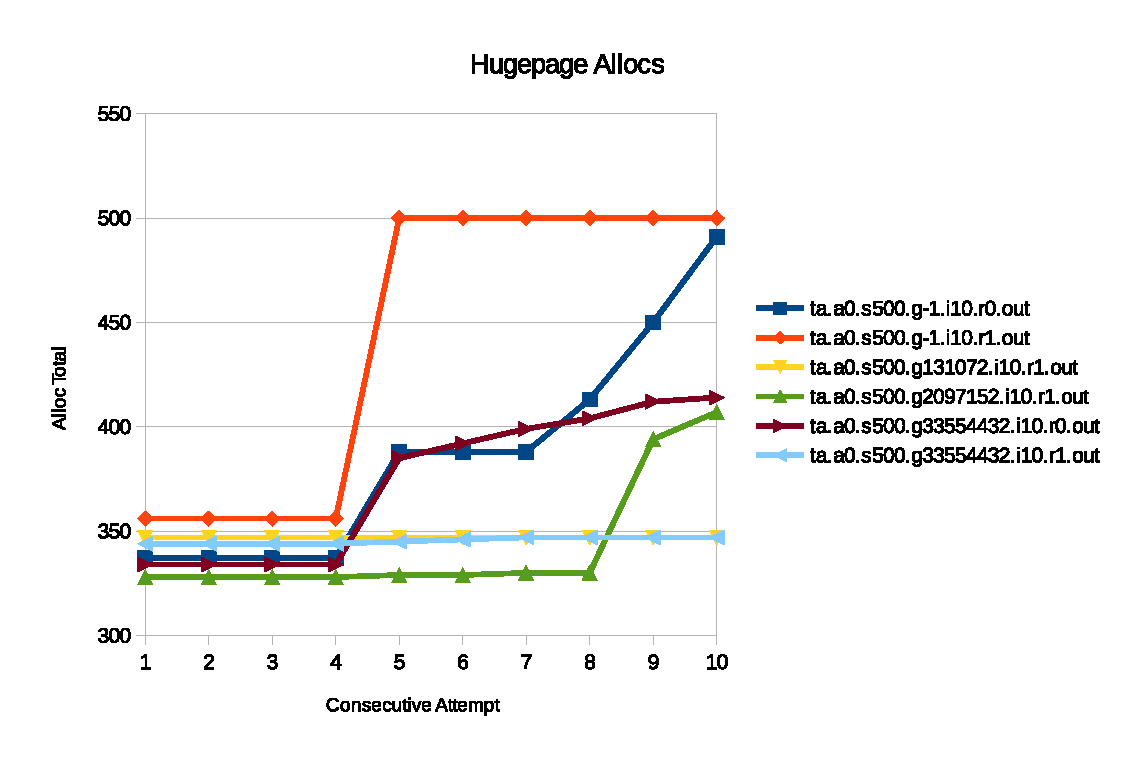
\includegraphics[width=\linewidth]{./datums/default_alloc.eps}
	\label{fig:default_alloc}
\end{figure}
\ref{fig:default_alloc}

\begin{figure}[h!]
	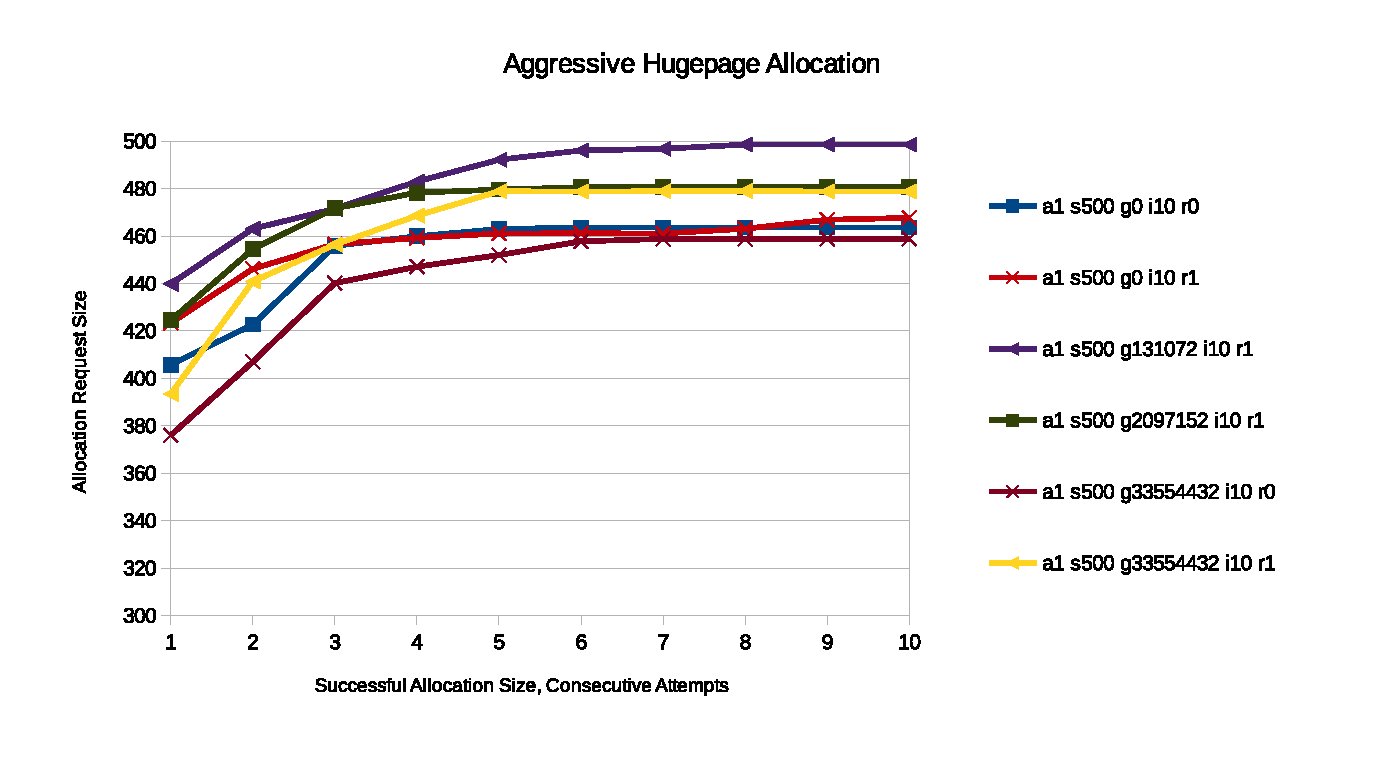
\includegraphics[width=\linewidth]{./datums/aggressive_alloc.eps}
	\label{fig:aggressive_alloc}
\end{figure}
\ref{fig:aggressive_alloc}

\section{Postamble}
\section{Future Works}
\begin{appendices}
	\newpage
	\chapter{Appendix 1: Table}
		\section{Data Table}
		\begin{table}[h!]
			\caption{Hugepage Allocation Data Points}
			\label{table1}
				%some stuff goes here
			\end{table}
	\chapter{Appendix 2: List of Figures}
		\listoffigures
\end{appendices}
\end{document}